%%%%%%%%%%%%%%%%%%%%%%%%%%%%%%%%%%%%%%%%%%%%%%%%%%%%%%%%%%%%
%%%%%%%%%%%%%%%%%%%%%%%%%%%%%%%%%%%%%%%%%%%%%%%%%%%%%%%%%%%%
%  Regret minimization and online gradient descent 
%%%%%%%%%%%%%%%%%%%%%%%%%%%%%%%%%%%%%%%%%%%%%%%%%%%%%%%%%%%%
%%%%%%%%%%%%%%%%%%%%%%%%%%%%%%%%%%%%%%%%%%%%%%%%%%%%%%%%%%%%
\chapter{
    %Generalization and Non-Smooth Optimization
    泛化与非光滑优化
    } \label{chap:first order}
\chaptermark{
%Generalization
泛化
}

%In previous chapter we have introduced the framework of mathematical optimization within the context of machine learning. We have described the mathematical formulation of several machine learning problems, notably training neural networks, as optimization problems. We then described as well as analyzed the most useful optimization method to solve such formulations: stochastic gradient descent.
在前一章中,我们介绍了机器学习背景下的数学优化框架。我们已经将几个机器学习问题的数学公式描述为优化问题,尤其是训练神经网络。然后,我们描述并分析了求解此类公式最有用的优化方法:随机梯度下降法。

%However, several important questions arise:
然而,出现了几个重要问题:
\begin{enumerate}
\item
%SGD was analyzed for smooth functions. Can we minimize non-smooth objectives?  
对SGD进行平滑函数分析。我们能将非平稳目标最小化吗?

\item
%Given an ERM problem (a.k.a. learning from examples, see first chapter), what can we say about generalization to unseen examples?  How does it affect optimization?
考虑到一个ERM问题(也就是从例子中学习,见第一章),我们能说些什么来概括看不见的例子?它如何影响优化?

\item 
%Are there faster algorithms than SGD in the context of ML?
在ML中,有没有比SGD更快的算法?

\end{enumerate}

%In this chapter we address the first two, and devote the rest of this manuscript/course to the last question.  
在本章中,我们将讨论前两个问题,并将本手稿/课程的其余部分用于最后一个问题。

%How many examples are needed to learn a certain concept? This is a fundamental question of statistical/computational learning theory that has been studied for decades (see end of chapter for bibliographic references). 
学习一个概念需要多少个例子?这是统计/计算学习理论的一个基本问题,已经研究了几十年(参考书目见本章末尾)。

%The classical setting of learning from examples is statistical. It assumes examples are drawn i.i.d from a fixed, arbitrary and unknown distribution. The mathematical optimization formulations that we have derived for the ERM problem assume that we have sufficiently many examples, such that optimizing a certain predictor/neural-network/machine on them will result in a solution that is capable of generalizing to unseen examples.  The number of examples needed to generalize is called the {\it sample complexity} of the problem, and it depends on the concept we are learning as well as the hypothesis class over which we are trying to optimize.
从例子中学习的经典设置是统计学。统计学假设样本是独立同分布的从某一固定的、任意的和未知的分布中提取的。
我们为ERM问题推导的数学优化公式假设我们有足够多的样本,这样,在这些样本上优化某个预测器/神经网络/机器将得到一个能够推广到未知示例的解决方案。
泛化所需的样本数称为问题的{it 样本复杂度},它取决于我们学习的概念以及我们试图优化的假设类。

%There are dimensionality notions in the literature, notably the VC-dimension and related notions, that give precise bounds on the sample complexity for various hypothesis classes. In this text we take an algorithmic approach, which is also deterministic. Instead of studying sample complexity, which is non-algorithmic, we study algorithms for regret minimization. We will show that they imply generalization for a broad class of machines. 
文献中有维度概念,比如VC维度和相关概念,它们为各种假设类的样本复杂性提供了精确的界限。
在本讲义中,我们采用一种算法方法,也是确定性的。
我们不研究样本复杂度(这是非算法的),而是研究遗憾最小化算法。
我们将证明,它们可以导出着一大类机器的泛化。

\section{
	%A note on non-smooth optimization
	关于非光滑优化的一个注记
	}

%Minimization of a function that is both non-convex and non-smooth is in general hopeless, from an information theoretic perspective. The following image explains why. The depicted function on the interval $[0,1]$ has a single local/global minimum, and if the crevasse is narrow enough, it cannot be found by any method other than extensive brute-force search, which can take arbitrarily long.
从信息论的角度来看,最小化一个既非凸又非光滑的函数通常是没有希望的。下图解释了原因。区间$[0,1]$上描述的函数有一个局部/全局最小值,如果裂缝足够窄,除了广泛的暴力搜索之外,任何方法都无法找到它,这可能需要任意长的时间。

\begin{figure}[h!]
\begin{center}
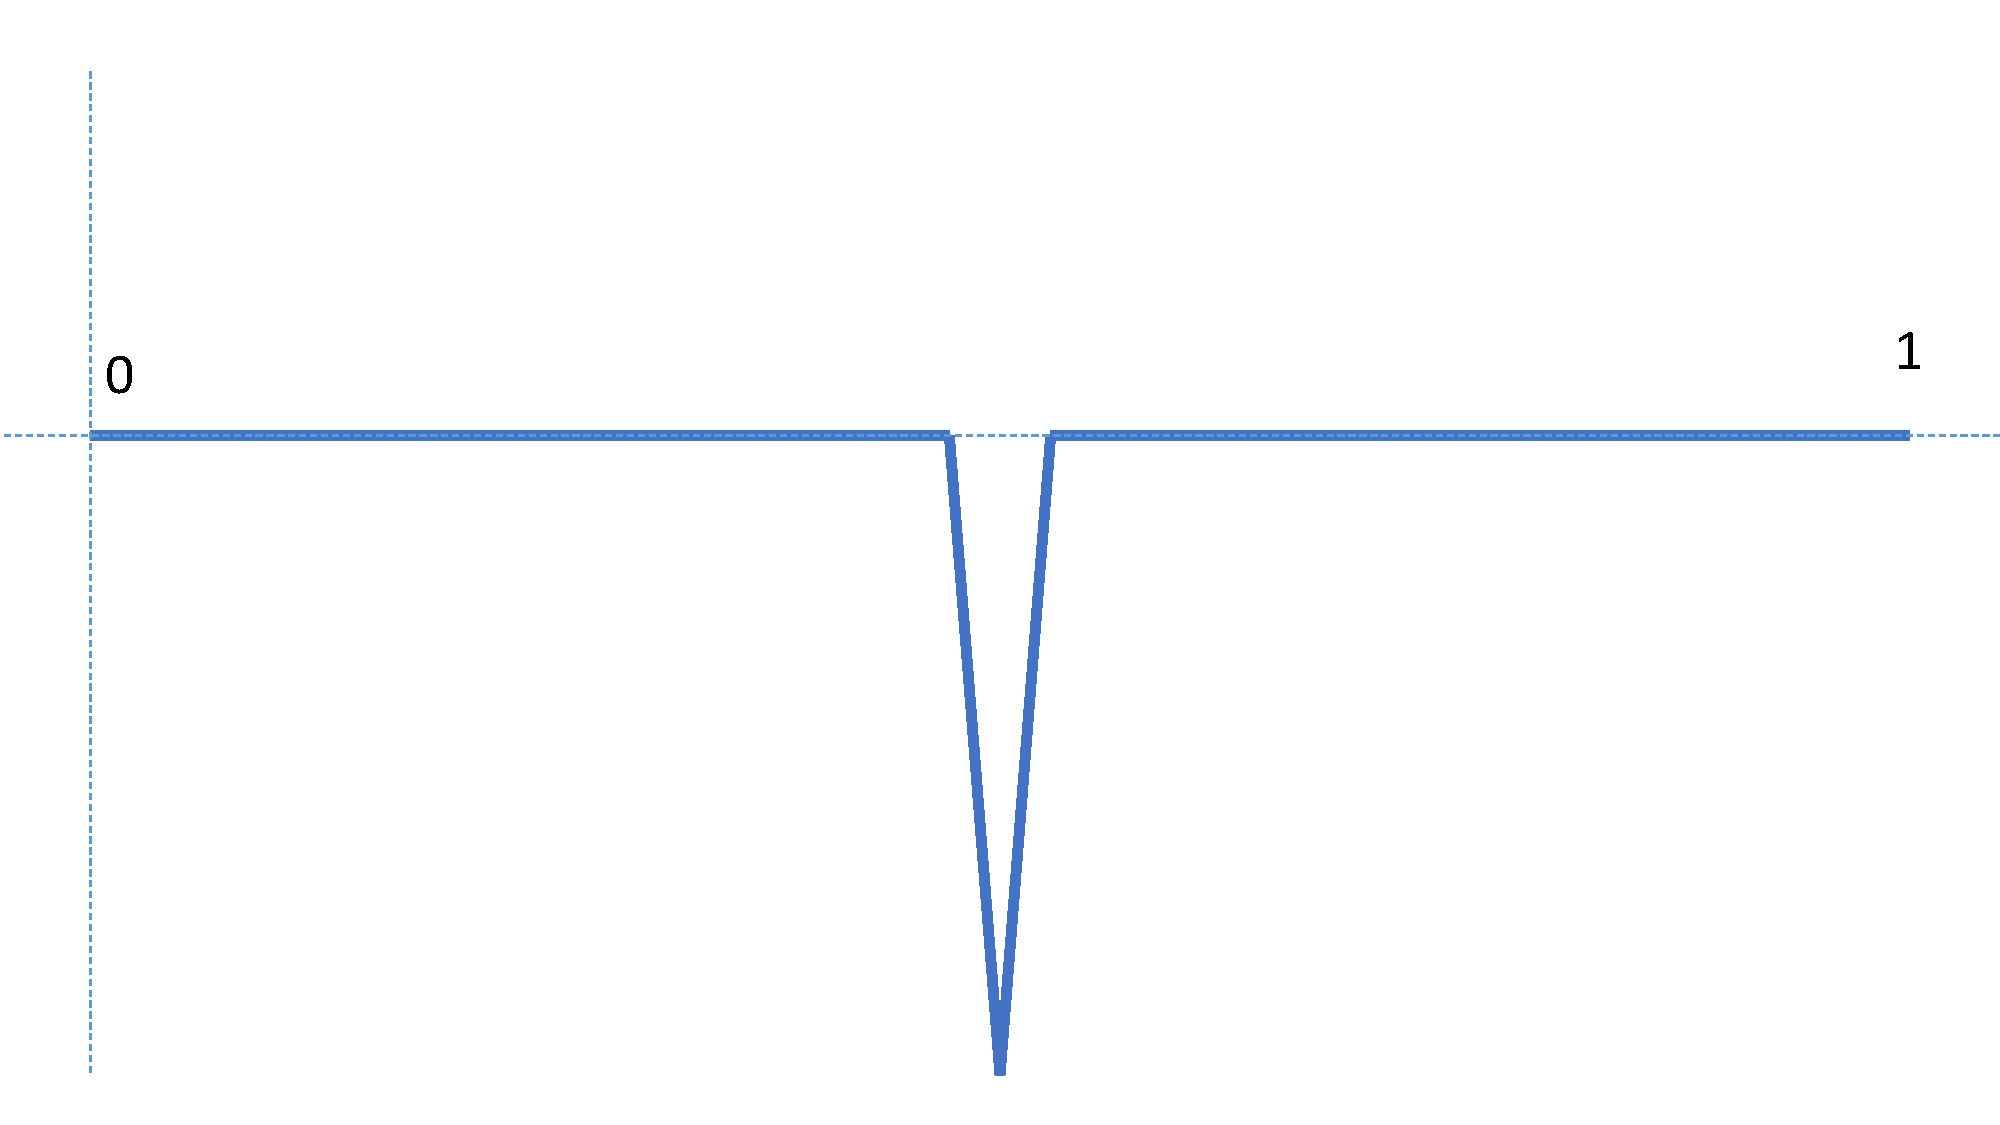
\includegraphics[width=3in]{figs/nonsmooth}
\end{center}
\caption{
	%Intractability of nonsmooth optimization 
	非光滑优化的难解性
	\label{fig:nonsmooth}}
\end{figure}


%Since non-convex and non-smooth optimization is hopeless, in the context of non-smooth functions we only consider  {\bf  convex} optimization. 
由于非凸和非光滑优化是无望的,在非光滑函数的情况下,我们只考虑{\bf 凸}优化。

\section{
	%Minimizing Regret
	减少遗憾
	} 


%The setting we consider for the rest of this chapter is that of online (convex) optimization. In this setting a learner iteratively predicts a point $\x_t \in \K$ in a convex set $\K \subseteq \reals^d$, and then receives a cost according to an adversarially chosen convex function $f_t \in \F$ from family $\F$.
我们在本章剩余部分考虑的设置是在线(凸)优化。在此设置中,学习者迭代地预测凸集 $\K \subseteq \reals^d$ 中的点 $\x_t \in \K$,然后根据从函数族 $\F$中逆向选择的凸函数 $f_t \in \F$ $\F$ 获得代价函数。

%The goal of the algorithms introduced in this chapter is to minimize worst-case {\it regret}, or difference between total cost and that of best point in hindsight:
本章中介绍的算法的目标是最小化最坏情况{\it 遗憾},或总成本与事后最佳点之间的差异:
$$ \regret = \sup_{f_1,...,f_T \in \F} \left\{ \sum_{t=1}^{T} f_t(\bx_t) -\min_{\bx \in \K}\sum_{t=1}^{T} f_t(\bx) \right\} . $$


%In order to compare regret to optimization error it is useful to consider the average regret, or ${\regret}/{T} $. Let  $\bar{\x}_T = \frac{1}{T} \sum_{t=1}^T \x_t$ be the average decision. If the functions $f_t$ are all equal to a single function $f : \K\mapsto \reals$, then Jensen's inequality implies that $f( \bar{\x}_T)$ converges to $f(\x^\star)$ if the average regret is vanishing, since
为了比较后悔和优化错误,考虑平均后悔或  ${\regret}/{T} $ 是很有用的。设 $\bar{\x}_T = \frac{1}{T} \sum_{t=1}^T \x_t$ 为平均决策。如果函数 $f_t$ 都等于单个函数 $f : \K\mapsto \reals$,那么Jensen不等式意味着如果平均遗憾逐渐消失,那么 $f( \bar{\x}_T)$ 收敛到 $f(\x^\star)$,因为
$$ f(\bar{\x}_T) - f(\x^\star ) \leq \frac{1}{T} \sum_{t=1} ^T [f(\x_t)  - f(\x^\star) ] = \frac{\regret}{T} $$ 


\section{
	%Regret implies generalization
	遗憾意味着泛化
	}

%Statistical learning theory for learning from examples postulates that examples from a certain concept are sampled i.i.d. from a fixed and unknown distribution. The learners' goal is to choose a hypothesis from a certain hypothesis class that can generalize to unseen examples. 
从样本中学习的统计学习理论假设,来自某个概念的样本是从固定的未知分布中进行独立同分布抽样来的。学习者的目标是从某个假设类中选择一个可以推广到未知的样本的假设。

%More formally, let $\D$ be a distribution over labelled examples $\{\ba_i  \in \reals^d , b_i \in \reals\} \sim \D$. Let $\H = \{ \x \} \ , \ \x: \reals^d \mapsto \reals$ be a hypothsis class over which we are trying to learn (such as linear separators, deep neural networks, etc.). The {\it generalization error} of a hypothesis is the expected error of a hypothesis over randomly chosen examples according to a given loss function $\ell : \reals \times \reals \mapsto \reals$, which is applied to the prediction of the hypothesis and the true label, $\ell(\x(\ba_i) , b_i)$.  Thus,
更形式化地表达就是,让 $\D$ 是标注样本 $\{\ba_i  \in \reals^d, b_i \in \reals\} \sim \D$ 上的分布。让 $\H = \{ \x \} \ , \ \x: \reals^d \mapsto \reals$ 成为一个我们试图学习的假设类(如线性分隔器、深层神经网络等)。假设的{\it 泛化误差}是根据给定的损失函数 $\ell : \reals \times \reals \mapsto \reals$在随机选择的样本上假设的预期误差,该函数用于预测假设和真实标签 $\ell(\x(\ba_i) , b_i)$。因此
$$ \err( \x) = \E_{\ba_i , b_i \sim \D} [ \ell (\x(\ba_i) , b_i ) ] .$$

%An algorithm that attains sublinear regret over the hypothesis class $\H$, w.r.t. loss functions given by $f_t(\x) = f_{\ba,b} (\x) = \ell( \x(\ba) , b)$, gives rise to a generalizing hypothesis as follows. 
在关于损失函数 $f_t(\x) = f_{\ba,b} (\x) = \ell( \x(\ba) , b)$ 的假设类$\H$上 一个算法获得次线性遗憾收敛速率,由此产生了如下一般化假设。

\begin{lemma}
%Let $\xbar =  \x_t$ for $t \in [T] $ be chose uniformly at random from $\{\x_1,...,\x_T\}$.%, and assume $f(\x)$ is convex. 
%Then, with expectation taken over random choice of $\xbar$ as well as choices of $f_t \sim \D$,
让  $\xbar =  \x_t$, $t \in [T] $ 从  $\{\x_1,...,\x_T\}$ 中均匀随机选择。%假设$f(\x)$是凸的。
然后,随着期望值取代了 $\xbar$ 的随机选择以及 $f_t \sim \D$ 的选择,
$$ \E [ \err(\bar{\x}) ]  \leq \E [ \err(\x^* ) ]  +  \frac{\regret}{T} $$
\end{lemma}
\begin{proof}[证明]
%By random choice of $\xbar$, we have
通过随机选择 $\xbar$,我们有:
$$ \E [ f(\xbar) ] =  \E\left[ \frac{1}{T} \sum_t f(\x_t) \right]$$
%Using the fact that $f_t \sim \D$, we have
使用  $f_t \sim \D$ 这个事实,我们有:
\begin{eqnarray*}
\E  [ \err(\xbar) ]  & = \E_{f \sim \D} [ f(\xbar)]  \\
& =  \E_{f_t} [ \frac{1}{T} \sum_t  f_t(\x_t)]  \\
& \leq  \E_{f_t} [ \frac{1}{T} \sum_t  f_t(\x^\star) ]  + \frac{\regret}{T} \\
& =  \E_{f} [ f(\x^\star) ]  + \frac{\regret}{T} \\
& = \E_f [ \err(\x^\star)] + \frac{\regret}{T} 
\end{eqnarray*}
\end{proof}
 



\section{
%Online gradient descent
在线梯度下降
} \label{section:ogd}

%Perhaps the simplest algorithm that applies to the most general setting of online convex optimization is online gradient descent.
%This algorithm is an online version of  standard gradient descent for offline optimization we have seen in the previous chapter.
%Pseudo-code for the algorithm is given in Algorithm \ref{figure:ogd}, and a conceptual illustration is given in Figure \ref{fig:ogd}.
也许适用于在线凸优化最普遍情形的最简单的算法是在线梯度下降。
该算法是我们在前一章中看到的用于离线优化的标准梯度下降的在线版本。
算法的伪代码在算法~\ref{figure:ogd}中给出,概念性说明在图~\ref{fig:ogd}中给出。

\begin{figure}[h!] 
	\begin{center}
		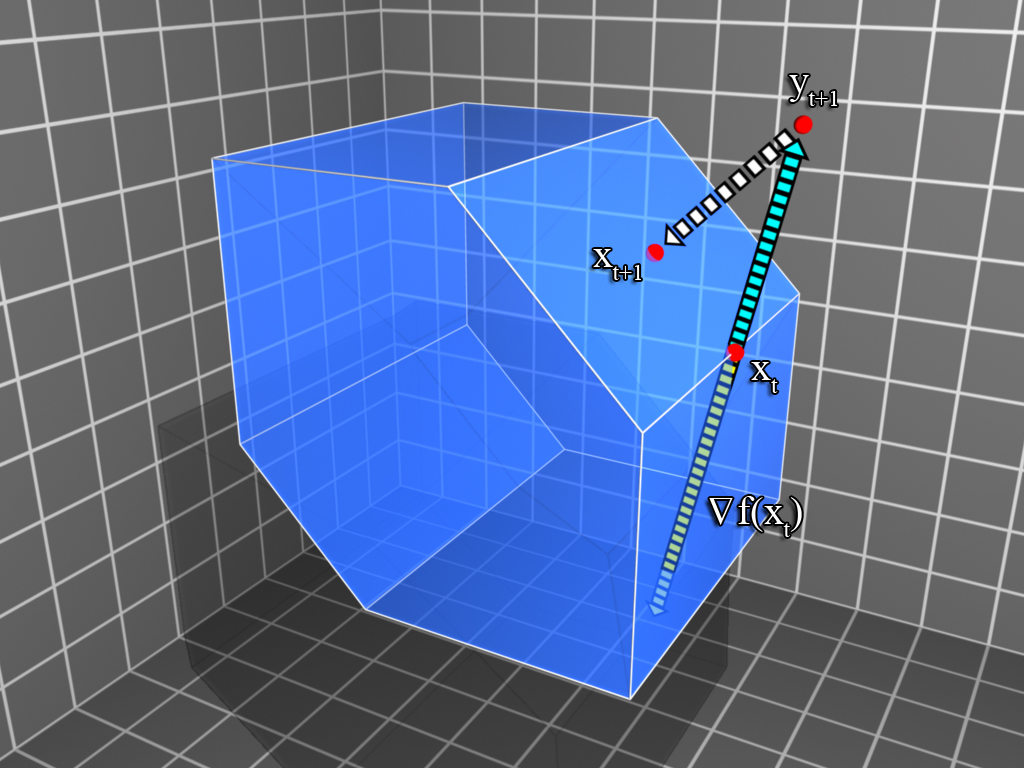
\includegraphics[width=4in]{figs/fig_gd_poly3}
	\end{center}
	\caption{
		%Online gradient descent: the iterate $\x_{t+1}$ is derived by advancing $\x_t$ in the direction of the current gradient $\nabla_t$, and projecting back into $\K$.
		在线梯度下降:迭代 $\x_{t+1}$是通过向当前梯度 $\nabla_t$ 的方向更新 $\x_t$ 并投影回 $\K$ 而得到的。
		\label{fig:ogd}
		}
\end{figure}

%In each iteration, the algorithm takes a step from the previous point in the direction of the gradient of the previous cost.  This step may  result in a point outside of the underlying convex set. In such cases, the algorithm projects the point back to the convex set, i.e. finds its closest  point in the convex set.
%Despite the fact that the next cost function may be completely different than the costs observed thus far, the regret attained by the algorithm is sublinear. This is formalized in the following theorem (recall the definition of $G$ and $D$ from the previous chapter).
在每次迭代中,该算法从上一个点向此前代价的梯度方向迈出一步。这一步可能会产生在可行凸集之外的点。在这种情况下,该算法将点投影回凸集,即在凸集中找到其最近的点。
尽管下一个代价函数可能与迄今为止观察到的代价完全不同,但该算法得到的遗憾是次线性的。这在下面的定理中得到了形式化(回想一下上一章中$G$和$D$的定义)。




\begin{algorithm}[h!]
		\caption{\label{figure:ogd} \ogd }
		\begin{algorithmic}[1]
			\STATE %Input: convex set $\K$, $T$, $\x_1 \in \mathcal{K}$, step sizes $\{ \eta_t \}$
			输入: 凸集合 $\K$, $T$, $\x_1 \in \mathcal{K}$, 步长 $\{ \eta_t \}$
			\FOR {$t=1$ to $T$}
			%\STATE Play $\x_t$ and observe cost $f_t(\x_t)$. 
			\STATE 输入 $\x_t$ 观测代价 $f_t(\x_t)$.
			%\STATE Update and project:
			\STATE 更新并投影:
			\begin{align*}
			& \y_{t+1} = \bx_{t}-\eta_{t} \nabla f_{t}(\bx_{t}) \\
			& \bx_{t+1} = \proj_\K(\y_{t+1})
			\end{align*}
			\ENDFOR
		\end{algorithmic}
\end{algorithm}
	




\begin{theorem}\label{thm:gradient}
%Online gradient descent with step sizes $\{\eta_t = \frac{D}{G \sqrt{t}} , \ t \in [T] \}$ guarantees the following for all $T \geq 1$:
步长为 $\{\eta_t = \frac{D}{G \sqrt{t}} , \ t \in [T] \}$ 的在线梯度下降为所有$T \geq 1$ 提供以下保证:
$$ \regret_T = \sum_{t=1}^{T} f_t(\bx_t) -\min_{\bx^\star \in \K}\sum_{t=1}^{T}
f_t(\bx^\star)\ \leq  {3} {G D}\sqrt{T} $$
\end{theorem}


\begin{proof}[证明]
%Let 
令
$\bx^\star \in \argmin_{\bx \in \K} \sum_{t=1}^T f_t(\bx)$.
%Define
定义
$\nabla_t \equaltri \nabla f_{t}(\bx_{t})$. 
%By convexity
根据凸性质:
\begin{eqnarray}  \label{eqn:gradient_inequality}
f_t(\bx_t) - f_t(\bx^\star) \leq   \nabla_t^\top (\bx_t - \bx^\star)
\end{eqnarray}
%We first  upper-bound $\nabla_t^\top (\bx_t-\bx^\star)$ using the update rule for $\bx_{t+1}$ and Theorem  \ref{thm:pythagoras} (the Pythagorean theorem):
我们首先使用 $\bx_{t+1}$ 和定理\ref{thm:pythagoras}(勾股定理)的更新规则来确定上界 $\nabla_t^\top (\bx_t-\bx^\star)$:
\begin{equation} \label{eqn:ogdtriangle}
\| \bx_{t+1}-\bx^\star \|^2\ =\  \left\|\proj_\K (\bx_t - \eta_t
\nabla_{t}) -\bx^\star\right\|^2 \leq  \left\|\bx_t - \eta_t \nabla_t-\bx^\star\right\|^2
\end{equation}

%Hence,
因此
\begin{eqnarray} \label{eqn:ogd_eq2}
\|\bx_{t+1}-\bx^\star\|^2\ &\leq&\ \|\bx_t- \bx^\star\|^2 + \eta_t^2
\|\nabla_t\|^2 -2 \eta_t \nabla_t^\top (\bx_t -\bx^\star)\nonumber\\
2 \nabla_t^\top (\bx_t-\bx^\star)\ &\leq&\ \frac{ \|\bx_t-
\bx^\star\|^2-\|\bx_{t+1}-\bx^\star\|^2}{\eta_t} + \eta_t G^2
\end{eqnarray}
%Summing \eqref{eqn:gradient_inequality} and \eqref{eqn:ogd_eq2}  from $t= 1$ to $T$, and setting
将 \eqref{eqn:gradient_inequality} 和 \eqref{eqn:ogd_eq2} 从 $t= 1$ 加到 $T$,并设
$\eta_t = \frac{D}{G \sqrt{t}}$ (
%with
取
$\frac{1}{\eta_0} \equaltri 0$):
\begin{align*}
& 2 \left( \sum_{t=1}^T f_t(\bx_t)-f_t(\bx^\star) \right ) \leq 2\sum_{t=1}^T \nabla_t^\top (\xv - \x^\star) \\
&\leq  \sum_{t=1}^T \frac{ \|\bx_t-
	\bx^\star\|^2-\|\bx_{t+1}-\bx^\star\|^2}{\eta_t} + G^2 \sum_{t=1}^T \eta_t    \\
&\leq  \sum_{t=1}^T \|\bx_t - \bx^\star\|^2 \left(
\frac{1}{\eta_{t}} -
\frac{1}{\eta_{t-1}} \right) + G^2 \sum_{t=1}^T \eta_t & \frac{1}{\eta_0} \equaltri 0, \\
& &  \|\xv[T+1] - \xv[]^* \|^2 \geq 0 \\
&\leq D^2 \sum_{t=1}^T \left(
\frac{1}{\eta_{t}} -
\frac{1}{\eta_{t-1}} \right) + G^2 \sum_{t=1}^T \eta_t \\
& \leq  D^2  \frac{1}{\eta_{T}}  + G^2 \sum_{t=1}^T \eta_t  & \mbox{ telescoping series } \\
& \leq 3 DG \sqrt{T}.
\end{align*}
%The last inequality follows since 
最后一个不等式成立是因为:
$\eta_t = \frac{D}{G \sqrt{t}}$ ,$\sum_{t=1}^T \frac{1}{\sqrt{t}} \leq 2 \sqrt{T}$.
\end{proof}


%The \ogd algorithm is straightforward to implement, and updates take linear time given the gradient. However, there is a projection step which may take significantly longer. 
\ogd 算法很容易实现,并且在给定梯度的情况下,更新只需要线性时间。然而,迭代过程中有一个投影步骤可能需要更长的时间。







\section{
	%Lower bounds
	下界
	} \label{section:lowerbound}



\begin{theorem} \label{thm:lowerbound}
%Any algorithm for online convex optimization incurs $\Omega(DG \sqrt{T})$ regret in the worst case. This is true even if  the cost functions are generated from a fixed stationary distribution.
任何在线凸优化算法在最坏的情况下都会产生 $\Omega(DG \sqrt{T})$ 遗憾。即使成本函数是由固定的平稳分布生成的,该结论仍成立。
\end{theorem}

%We give a sketch of the proof; filling in all details is left as an exercise at the end of this chapter. 
我们给出了证明的框架;填写所有细节将作为本章末尾的练习。

%Consider an instance of OCO where the convex set $\K$ is the $n$-dimensional hypercube, i.e.
考虑OCO的一个例子,其中凸集 $\K$ 是 $n$ 维超立方体,即
$$ \K = \{ \bx \in \reals^n \ , \  \|\bx\|_\infty \leq 1 \}.$$
%There are $2^n$ linear cost functions, one for each vertex $\bv \in \{\pm 1\}^n$, defined as
有 $2^n$ 线性成本函数,每个顶点$\bv \in \{\pm 1\}^n$,定义为
$$ \forall \bv \in \{ \pm 1 \}^n \ , \ f_\bv(\bx)  = \bv^\top \bx. $$
%Here, the cost functions are linear:  they are inner products with  vectors which are  vertices of the hypercube. 
%Notice that both the diameter of $\K$ and the bound on the norm of the cost function gradients, denoted G, are bounded by
请注意,$\K$的直径和代价函数梯度范数的界(表示为G) 均由下式限定:
$$  D \leq \sqrt{ \sum_{i=1}^n 2^2 } = 2 \sqrt{n} , \ G = \sqrt{ \sum_{i=1}^n (\pm1)^2 } = \sqrt{n}  $$

%The cost functions in each iteration are chosen at random, with uniform probability, from the set
每次迭代中的代价函数都是随机选择的,概率是一致的,来自集合:
$\{ f_\bv , \bv \in \{\pm 1\}^n \}$. 
%Denote by $\bv_t \in \{\pm 1\}^n $ the vertex chosen in iteration $t$, and denote $f_t = f_{\bv_t}$. By uniformity and independence, for any $t$ and $\bx_t$ chosen online,
在迭代 $t$ 中,选取的点表示为 $\bv_t \in \{\pm 1\}^n $,记 $f_t = f_{\bv_t}$。通过均匀独立的方式,对任意 $t$ 和 在线选择的$\bx_t$,
$\E_{\bv_t}[f_{t}(\bx_t)]= \E_{\bv_t}[ \bv_t^\top
\bx_t] = 0$. 
%However,
然而
\begin{align*}
\E_{\bv_1,\ldots,\bv_T}\left[\min_{\bx \in \K} \sum_{t=1}^T f_t(\bx)\right] & =
\E \left[\min_{\bx \in \K} \sum_{i \in [n]} \sum_{t=1}^T \bv_t(i) \cdot \bx_i \right] \\
& = n \E\left[-\left|\sum_{t=1}^T \bv_t(1) \right|\right] & \mbox{i.i.d. coordinates}\\
& = -\Omega(n \sqrt{T}).
\end{align*}
%The last equality is left as exercise \ref{exercise:ogd-lower-bound}. 
最后一个等式保留为练习题 \ref{exercise:ogd-lower-bound}。

%The facts above nearly complete the proof of Theorem \ref{thm:lowerbound}; see the exercises at the end of this chapter. 
上述事实几乎完成了定理\ref{thm:lowerbound}的证明;参见本章末尾的练习。




\section{
	%Online gradient descent for strongly convex functions
	强凸函数的在线梯度下降
	} \label{section:ogdnew}


%The first algorithm that achieves regret logarithmic in the number of iterations is a twist on the online gradient descent algorithm, changing only the step size. The following theorem establishes logarithmic bounds on the regret if the cost functions are strongly convex.
第一个迭代次数达到对数的算法是对在线梯度下降算法的一种改进,只改变了步长。如果代价函数是强凸的,下面的定理建立了遗憾的对数界。

\begin{theorem}\label{thm:gradient2}
%For  $\alpha$-strongly convex loss functions, 
%\ogd with step sizes $\eta_t = \frac{1}{\alpha {t}}$ achieves the
%following guarantee for all $T \geq 1$
对于$\alpha$-强凸损失函数,
步长为 $\eta_t = \frac{1}{\alpha {t}}$的\ogd,对所有$T\geq 1$ 有如下保证:
$$\regret_T\ \leq\  \sum_{t=1}^{T} \frac{1}{\alpha t} \|\nabla_t\|^2 \leq \frac{G^2}{2 \alpha}(1 + \log T).$$
\end{theorem}


\begin{proof}[证明]
%Let 
令
$\bx^\star \in \argmin_{\bx \in \K} \sum_{t=1}^T f_t(\bx)$.
%Recall the definition of regret 
根据遗憾最小化中遗憾的定义:
$$ \regret_T\ = \sum_{t=1}^{T} f_t(\bx_t) - \sum_{t=1}^{T} f_t(\bx^\star). $$


%Define $\nabla_t \equaltri \nabla f_t(\bx_t)$. Applying the definition of $\alpha$-strong convexity to the pair of points $\x_t$,$\x^*$, we have
定义  $\nabla_t \equaltri \nabla f_t(\bx_t)$。将 $\alpha$-强凸性的定义应用于 $\x_t$,$\x^*$ 点对,我们得到
\begin{eqnarray}
2(f_t(\bx_t)-f_t(\bx^\star)) &\leq& 2\nabla_t^\top (\bx_t-\bx^\star)-\alpha
\|\bx^\star-\bx_t\|^2.\label{eqsz}
\end{eqnarray}
%We proceed to upper-bound $\nabla_t^\top (\bx_t-\bx^\star)$. 
%Using the update rule for $\bx_{t+1}$ and the Pythagorean theorem \ref{thm:pythagoras}, we get
我们得到上界 $\nabla_t^\top (\bx_t-\bx^\star)$。
使用  $\bx_{t+1}$ 的更新规则和勾股定理\ref{thm:pythagoras},我们得到
$$\| \bx_{t+1}-\bx^\star \|^2\ =\ \|\proj_\K(\bx_t - \eta_{t} \nabla_t)-\bx^\star\|^2 \leq  \|\bx_t - \eta_{t} \nabla_t-\bx^\star\|^2.$$
%Hence,
因此
\begin{eqnarray*}
\|\bx_{t+1}-\bx^\star\|^2\ &\leq&\ \|\bx_t- \bx^\star\|^2 + \eta_{t}^2
\|\nabla_t\|^2 -2
\eta_{t} \nabla_t^\top (\bx_t - \bx^\star)\nonumber\\
\end{eqnarray*}
%and
并有
\begin{eqnarray}
2 \nabla_t^\top (\bx_t-\bx^\star)\ &\leq&\ \frac{ \|\bx_t-
\bx^\star\|^2-\|\bx_{t+1}-\bx^\star\|^2}{\eta_{t}} + \eta_{t} \| \nabla_t\|^2.
\label{eqer}
\end{eqnarray}
%Summing  \eqref{eqer} from $t= 1$ to $T$, 
%setting $\eta_{t} = \frac{1}{\alpha t}$ (define $\frac{1}{\eta_0} \equaltri 0$),
%and combining with \eqref{eqsz}, we have:
从 $t=1$ 到 $T$ 将 \eqref{eqer} 相加,
设置 $\eta_{t} = \frac{1}{\alpha t}$ (定义$\frac{1}{\eta_0} \equaltri 0$),
结合\eqref{eqsz},我们有:
\begin{eqnarray*}
&  & 2 \sum_{t=1}^T (f_t(\bx_t)-f_t(\bx^\star) ) \\
&\leq &\
 \sum_{t=1}^T \|\bx_t-\bx^\star\|^2
\left(\frac{1}{\eta_{t}}-\frac{1}{\eta_{t-1}}-\alpha\right) + 
\sum_{t=1}^{T} \eta_{t} \|\nabla_t\|^2  \\
& & \mbox{ 
%since
因此
}  \frac{1}{\eta_0} \equaltri 0, \|\xv[T+1] - \xv[]^* \|^2 \geq 0 \\ \\
&=&\ 0 +  \sum_{t=1}^{T} \frac{1}{\alpha t} \|\nabla_t\|^2 \\
& \leq &  \frac{G^2}{\alpha}(1 + \log T )
\end{eqnarray*}
\end{proof}


\section{
	%Online Gradient Descent implies SGD
	在线梯度下降意味着SGD
	}

%In this section we notice that OGD and its regret bounds imply the SGD bounds we have studied in the previous chapter. The main advantage are the guarantees for non-smooth stochastic optimization, and constrained optimization. 
在本节中,我们注意到OGD及其遗憾界暗示着我们在前一章中研究过的SGD界。其主要优点是保证了非光滑随机优化和约束优化。

%Recall that in stochastic optimization, the optimizer attempts to minimize a convex function over a convex domain as given by the mathematical program:
回想一下,在随机优化中,优化器试图最小化凸域上的凸函数,如下数学规划:
\begin{align*}
\min_{\x \in \K } f(\x). 
\end{align*}
%However, unlike standard offline optimization, the optimizer is given access to a noisy gradient oracle, defined by
然而,与标准的离线优化不同,优化器可以访问含噪梯度预言器,定义如下:
$$ \mathcal{O}(\x) \equaltri \tilde{\nabla }_\x  \ \mbox{ s.t. } \  \E[\tilde{\nabla }_\x ] = \nabla f(\x) \ , \   \E[ \|\tilde{\nabla }_\x\|^2 ] \leq G^2  $$
%That is, given a point in the decision set, a noisy gradient oracle returns a random vector whose expectation is the gradient at the point and whose second moment is bounded by $G^2$. 
也就是说,给定决策集中的一个点,含噪梯度预言器返回一个随机向量,其期望值是该点的梯度,其二阶矩以$G^2$为界。
	
%We will show that regret bounds for OCO  translate to convergence rates for stochastic optimization.  As a special case, consider the online gradient descent algorithm whose regret is bounded by 
我们将证明OCO的遗憾界转化为随机优化的收敛速度。作为特例,考虑在线梯度下降算法,其遗憾有界于
$$\regret_{T} = O(DG\sqrt{T}) $$
%Applying the OGD algorithm over a sequence of linear functions that are defined by the noisy gradient oracle at consecutive points, and finally returning the average of all points along the way, we obtain the stochastic gradient descent algorithm, presented in Algorithm \ref{alg:sgd}.
将OGD算法应用于连续点上由噪声梯度预言器定义的线性函数序列,并最终返回沿途所有点的平均值,我们得到了随机梯度下降算法,如算法\ref{alg:sgd}中所示。
\begin{algorithm}[h!]
\caption{
%stochastic  gradient descent
随机梯度下降
}
\label{alg:sgd}
\begin{algorithmic}[1]
%\STATE Input: $f$, $\K$, $T$, $\x_1 \in \mathcal{K}$, step sizes $\{ \eta_t \}$
\STATE 输入: $f$, $\K$, $T$, $\x_1 \in \mathcal{K}$, 步长 $\{ \eta_t \}$
\FOR {$t=1$ to $T$}
\STATE \label{alg:sgd-defnft} Let $\tilde{\nabla}_t = \mathcal{O}(\x_t)$ and define: $ f_t(\x) \equaltri  \langle \tilde{\nabla}_t , \x \rangle $ 
%\STATE Update and project:
\STATE 更新并投影:
$$ \y_{t+1} = \bx_{t}-\eta_t \tilde{\nabla}_t$$
$$ \bx_{t+1} = \proj_\K(\y_{t+1})$$
\ENDFOR
\RETURN $\bar{\x}_T \equaltri \frac{1}{T} \sum_{t=1}^T \x_t$ 
\end{algorithmic}
\end{algorithm}
	

\begin{theorem} \label{thm:sgd}
%Algorithm \ref{alg:sgd} with step sizes $\eta_t = \frac{D}{G \sqrt{t}}$ guarantees
具有步长 $\eta_t = \frac{D}{G \sqrt{t}}$ 的算法  \ref{alg:sgd} 生成
$$ \E[ f(\bar{\x}_T) ]  \leq \min_{\x^\star \in \K } f(\x^\star) + \frac{3 GD }{\sqrt{T}}$$
\end{theorem}
\begin{proof}[证明]
%By the regret guarantee of OGD, we have
根据OGD的遗憾保证,我们有:
\begin{align*}
&  \E [ f(\bar{\x}_T) ] - f(\x^\star) \\
 & \leq \E [ \frac{1}{T} \sum_t  f(\x_t) ]  - f(\x^\star)  & \mbox{
%convexity of $f$ (Jensen) 
$f$ 的凸性质(Jensen)
}\\
&\leq \frac{1}{T}  \E [ \sum_t  \langle \nabla f(\x_t) , \x_t - \x^\star\rangle ] & \mbox{
convexity again
仍然是凸性质
}\\
& = \frac{1}{T} \E[ \sum_t \langle \tilde{\nabla}_t , \x_t -\x^\star \rangle ] & \mbox{
%noisy gradient estimator
含噪梯度估计器
}\\
& = \frac{1}{T} \E[ \sum_t  f_t( \x_t)  -f_t(\x^\star) ] & \mbox{ Algorithm \ref{alg:sgd}, line \eqref{alg:sgd-defnft} }\\
& \leq  \frac{\regret_T }{T} & \mbox{
%definition
定义
}\\
& \leq  \frac{3GD }{\sqrt{T}} & \mbox{ theorem \ref{thm:gradient}}
\end{align*}
\end{proof}
	
%It is important to note that in the proof above, we have used the fact that the regret bounds of \ogd hold against an adaptive adversary. This need arises since the cost functions $f_t$ defined in Algorithm \ref{alg:sgd} depend on the choice of decision $\x_t \in \K$. 
需要注意的是,在上面的证明中,我们使用了一个事实,即\ogd的遗憾界限在自适应对手时能够保持。这是由于算法\ref{alg:sgd}中定义的成本函数 $f_t$ 取决于决策 $\x_t \in \K$的选择。

%In addition, the careful reader may notice that by plugging in different step sizes (also called learning rates) and applying SGD to strongly convex functions, one can attain $\tilde{O}({1}/{T})$ convergence rates. Details of this derivation are left as exercise \ref{exercise:fast-rate}. 
此外,细心的读者可能会注意到,通过插入不同的步长(也称为学习率)并将SGD应用于强凸函数,可以获得  $\tilde{O}({1}/{T})$ 的收敛速度。此推导的详细信息保留为练习题\ref{exercise:fast-rate}。

\newpage
\section{
	%Exercises
	练习题}

\begin{enumerate}
\item \label{exercise:fast-rate}
	
%Prove that SGD for a strongly convex function can, with appropriate parameters $\eta_t$, converge as $\tilde{O}(\frac{1}{T})$.  You may assume that the gradient estimators have Euclidean norms bounded by the constant $G$.  
证明强凸函数的SGD在适当的参数$\eta_t$下可以收敛为 $\tilde{O}(\frac{1}{T})$。你可以假设梯度估计器的欧几里德范数以常数$G$为界。

\item
%Design an OCO algorithm that attains the same asymptotic regret bound as OGD, up to factors logarithmic in $G$ and $D$,  without knowing the parameters $G$ and $D$ ahead of time. 
设计一个OCO算法,在不提前知道参数$G$和$D$的情况下,实现与OGD相同的渐近遗憾界,最多可达关于$G$和$D$的对数级别。


\item \label{exercise:ogd-lower-bound}
%In this exercise we prove a tight lower bound on the regret of any algorithm for online convex optimization.
在本练习中,我们证明了在线凸优化算法的精确下界。
\begin{enumerate}
\item
%For any sequence of $T$ fair coin tosses, let $N_h$ be the number of head outcomes and $N_t$ be the number of tails. Give an asymptotically tight upper and lower bound on $\E[ \left| N_h - N_t \right|]$ (i.e., order of growth of this random variable as a function of $T$, up to multiplicative and additive constants). 
对于公平抛出硬币的任何 $T$ 序列,让 $N_h$ 为正面结果数,$N_T$为反面结果数。给出 $\E[ \left| N_h - N_t \right|]$ 上的渐近紧上界和下界(即该随机变量的增长阶为$T$的函数,直至乘法和加法常数)。
\item
%Consider a 2-expert problem, in which the losses are inversely correlated: either expert one incurs a loss of one and the second expert zero, or vice versa. Use the fact above to design a setting in which any experts algorithm incurs regret asymptotically matching the upper bound.
考虑一个2-专家的问题,其中损失是负相关的:一位专家的损失为1,另一位专家的损失为0,反之亦然。利用上述事实设计一个设置,在该设置中,任何专家算法都会产生与上界渐近匹配的遗憾。
\item
%Consider the general OCO setting over a convex set $\mathcal{K}$. Design a setting in which the cost functions have gradients whose norm is bounded by $G$, and obtain a lower bound on the regret as a function of $G$, the diameter of $\mathcal{K}$, and the number of game iterations.
考虑凸集 $\mathcal{K}$ 上的一般OCO设置。设计一个场景,其中代价函数具有范数以$G$为界的梯度,并获得遗憾的下界,作为$G$、$\mathcal{K}$ 的直径和迭代次数的函数。
\end{enumerate}
	

\end{enumerate}



\newpage
\section{
%Bibliographic remarks
书目注释
}

%The OCO framework was introduced by Zinkevich in \cite{Zinkevich03}, where the OGD algorithm was introduced and analyzed. Precursors to this algorithm, albeit for less general settings, were introduced and analyzed in \cite{KivWar97}. 
%Logarithmic regret algorithms for Online Convex Optimization were introduced and analyzed in \cite{HAK07}.  For more detailed exposition on this prediction framework and its applications see \cite{OCObook}.
Zinkevich在 \cite{Zinkevich03}中介绍了OCO框架,并对OGD算法进行了介绍和分析。该算法的前身,尽管不太通用,在\cite{KivWar97}中介绍和分析。
工作\cite{HAK07}介绍并分析了在线凸优化的对数遗憾算法。有关此预测框架及其应用程序的更多详细说明,请参见\cite{OCObook}。

%The SGD algorithm dates back to Robbins and Monro \cite{robbins1951}. Application of SGD to soft-margin SVM training was explored in \cite{Shalev-ShwartzSSC11}. Tight convergence rates of SGD for strongly convex and non-smooth functions were only recently obtained in \cite{hazan:beyond},\cite{RSS},\cite{SZ}.
SGD算法可以追溯到Robbins和Monro\cite{robbins1951}。在\cite{Shalev-ShwartzSSC11}中探讨了SGD在软边缘支持向量机训练中的应用。强凸和非光滑函数的SGD的紧收敛速度最近才在\cite{hazan:beyond},\cite{RSS},\cite{SZ}中得到。


